
%(BEGIN_QUESTION)
% Copyright 2006, Tony R. Kuphaldt, released under the Creative Commons Attribution License (v 1.0)
% This means you may do almost anything with this work of mine, so long as you give me proper credit

Explain how this motor control circuit works for an electrically-actuated gate valve.  Note the use of a three-position switch with ``Close,'' ``Off,'' and ``Open'' positions:

$$\includegraphics[width=15.5cm]{i01392x01.eps}$$

Specifically, explain why the upper limit switch is designed to open when it detects a certain amount of motor torque, and why the lower limit switch is designed to open when it detects a certain distance of valve stem travel.  It will help greatly to consider how a gate valve works when answering this question!

\vskip 20pt \vbox{\hrule \hbox{\strut \vrule{} {\bf Suggestions for Socratic discussion} \vrule} \hrule}

\begin{itemize}
\item{} Explain how to interpret the symbol used for the ``Close/Off/Open'' switch.
\item{} Explain what {\it arc flash} is, and how to protect yourself from it while working on high-voltage motor control circuits such as this one.
\end{itemize}

\underbar{file i01392}
%(END_QUESTION)





%(BEGIN_ANSWER)

When closing a gate valve, you want the gate to wedge firmly against the valve seat for tight shutoff.  However, it does not matter as much whether or not the gate is fully withdrawn when the valve is wide open.
 
%(END_ANSWER)





%(BEGIN_NOTES)

\vfil \eject

\noindent
{\bf Summary Quiz:}

Explain why motor-operated sliding-stem valves typically use a {\it torque} switch to stop valve motion when closing, rather than a ``travel'' switch.

\begin{itemize}
\item{} A torque switch saves energy by limiting the motor's effort while moving
\vskip 5pt 
\item{} A torque switch ensures the flange gaskets are properly tightened 
\vskip 5pt 
\item{} Torque switches are less expensive to install than travel switches
\vskip 5pt 
\item{} There is no good reason; it's just a tradition within the valve industry
\vskip 5pt 
\item{} A torque switch permits the motor to spin faster, reducing time to close
\vskip 5pt 
\item{} A torque switch ensures consistent seating of the valve when it closes
\end{itemize}


%INDEX% Final Control Elements, valve: electric actuator

%(END_NOTES)


